\documentclass[12pt]{article}
\usepackage{graphicx} %  inserting images
\usepackage{pdfpages}
\usepackage{setspace}
\usepackage{times}
\usepackage{xcolor}
\usepackage{amsmath, amssymb} % For better math
\usepackage{lmodern}   
\title{Signals and systems Lab 1}
\author{Denzel Onyango Ninga
ENG-219-042/2022}
\date{March 2025}

\begin{document}
\maketitle

\section{Abstract}
In this lab report, I will be able to analyze and explain the plots of specific signals: signum, rectangular, triangular, sinc, impulse,
step, square, discrete exponential, and discrete cosine.I will also analyze the relationship between frequencies for discrete cosine and exponential signals. I will State and verify the Cauchy-Schwarz inequality, Classify systems based on linearity, time-invariance, causality, and stability and perform advanced signal operations and analyze their properties.By use of MATLAB plot and calculate these , I'll verify.
\section{Introduction}
First off, a signal is a function representing a physical quantity or variable and a system is a mathematical model of a physical process that relates the input signal to the output signal. 
The origin of the word systems dates back to the 15th century, 
when it was used as a Latin word \textit{systema}, 
which means the entire universe.\footnote{Fatoş Tunay Yarman Vural and Emre Akbaş, 
\textit{Signals and Systems: Theory and Practical Explorations with Python} 
(CRC Press, 2022), p. 19.}
Signal and system concepts arise in a wide variety of areas, from home-oriented consumer electronics and multimedia entertainment products to sophisticated communications, aeronautics and astronautics, and control. Of course, signals and systems are the entire universe.Signals and systems are the backbone of communication.
\subsection{Lab Objectives}
The objectives of this lab are:
\begin{itemize}
    \item Understand and plot specific signals: signum, rectangular, triangular, sinc, impulse, step, square, discrete exponential, and discrete cosine.
    \item Use subplots to analyze the relationship between frequencies for discrete cosine and exponential signals.
    \item Calculate inner products of signals and use them to compute energy and power, comparing hand calculations with code results.
    \item State and verify the Cauchy-Schwarz inequality.
    \item Classify systems based on linearity, time-invariance, causality, and stability.
    \item Perform advanced signal operations and analyze their properties.
\end{itemize}

\section{Methodology}
Most of this lab was completing the skeleton codes provided in the Lab Manual 'Signal and System Analysis Lab 1'.I did this using MATLAB R2024b and I did use alternatives for certain codes since I just did not have certain toolboxes such as the rectangular Toolbox, so I used Rectangular function alternatively for rectangularPulse. It was a success. I ran all my codes in the live script in MATLAB, ran each section separately, making the necessary changes to ensure it was a success and of course it was.

Also, I did the hand calculations and verified the results.It was rough here as I was involved with finding the inner product and calculating the catchy-schwarz inequalities, thanks to Indian YouTubers-they are geniuses.The YouTube channel The grade Academy ,video titled 'Real Analysis lecture 10 -catchy-schwartz inequality Proof' was a life saver.\footnote{The Grade Academy, 
\textit{Real Analysis Lecture 10 - Cauchy-Schwarz Inequality Proof},YouTube,Published on[2021],\url{https://youtu.be/i851HnlBpv8?si=HBe9MPFa9HZwLYDF},accessed on [18/3/2025].} 
The methodology included:
\begin{itemize}
    \item Running MATLAB codes to generate and analyze signal plots.
     \item Reading necessary materials,including Textbooks to understand various concepts and just to cross check them.
    \item Watching YouTube videos to grasp the underlying concepts.
    \item Performing hand calculations to verify MATLAB results and ensure theoretical accuracy.
    \item Researching the internet .
\end{itemize}
\normalsize
\section{Results}
The results after completing or even making necessary improvements to the MATLAB skeleton codes and performing hand calcculations were as follows;
\subsection{MATLAB Code}
The MATLAB code used in this lab is provided below It contains the full implementation for generating and analyzing the signals:
\includepdf[pages=-, scale=0.9]{ninga.pdf}
\subsection{Hand calculations}
The hand calculations below aligned mostly with code results:
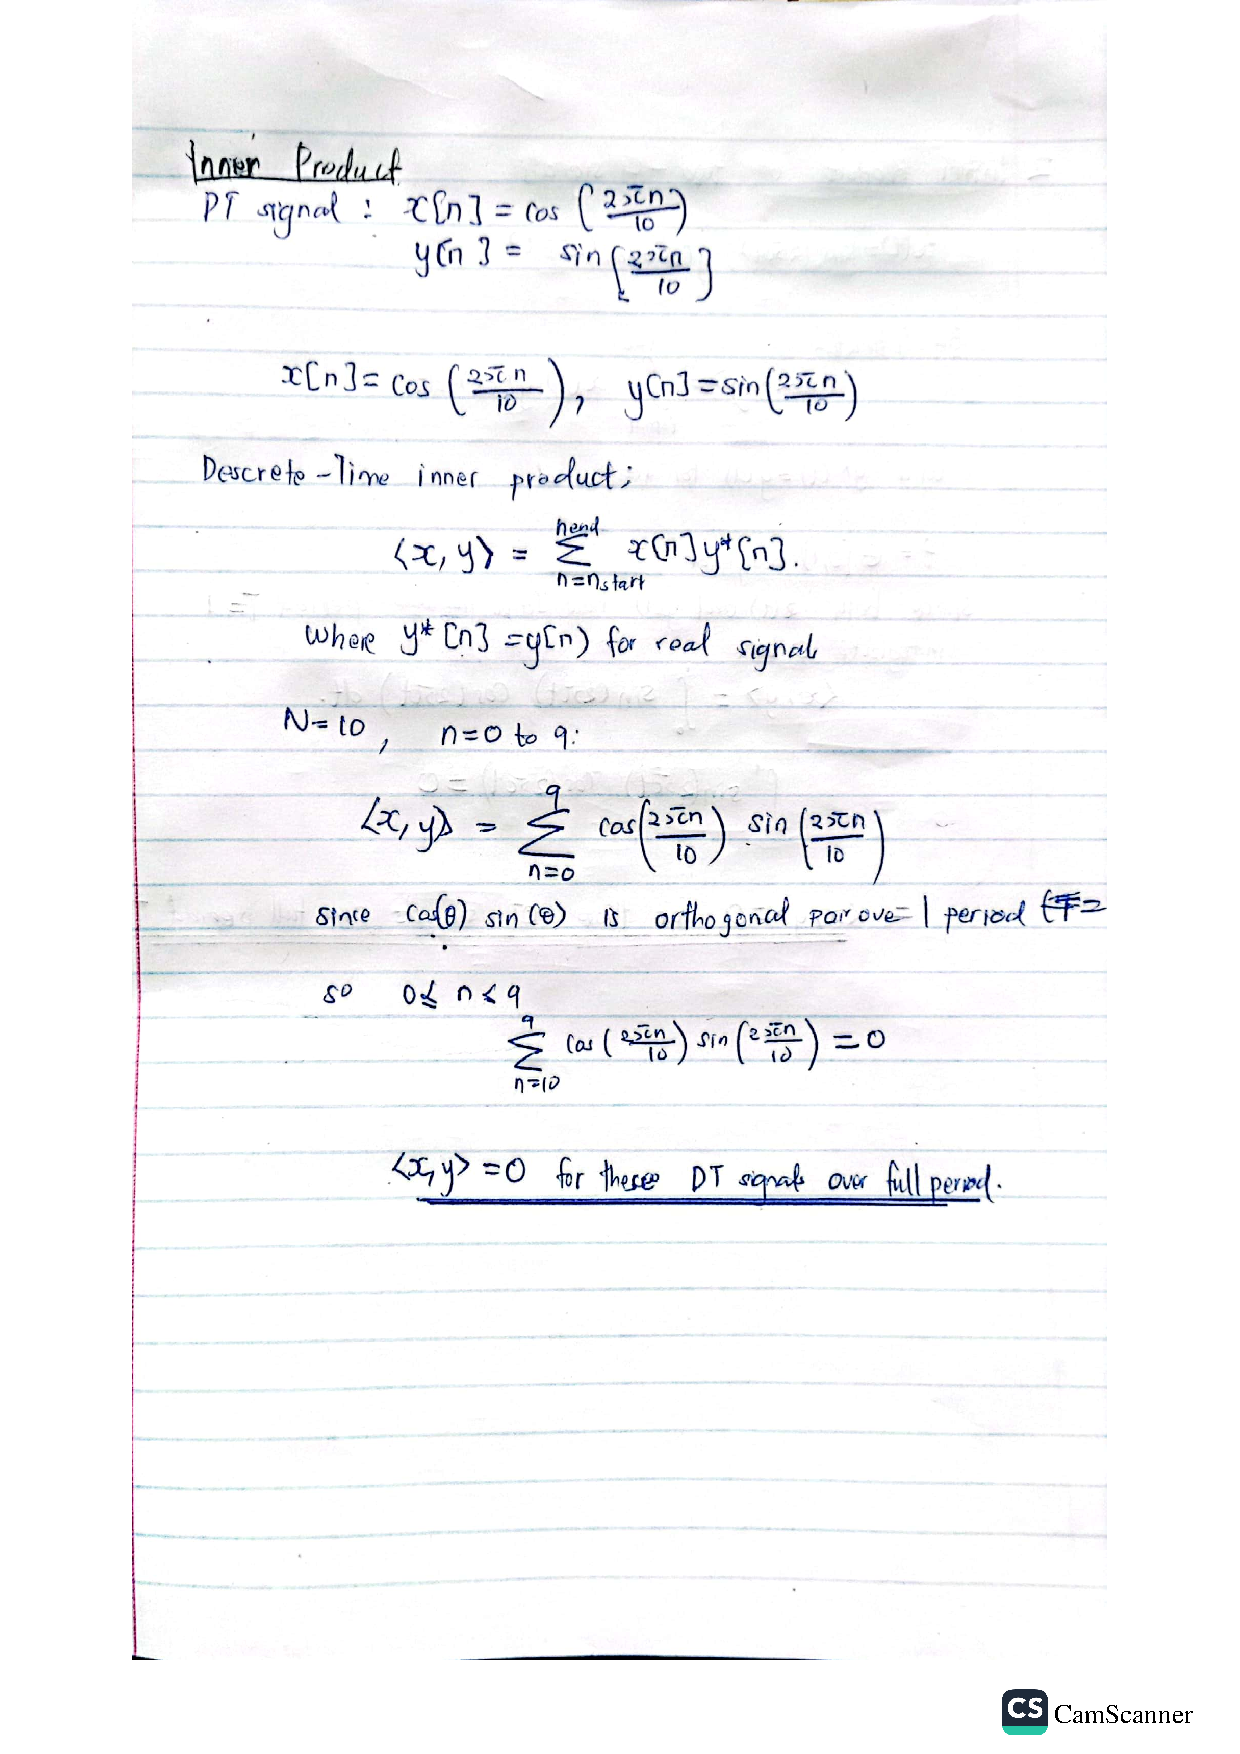
\includepdf[pages=-, scale=0.9]{hands.pdf}
\section{Discussions and Observations}

\subsection{Exercise 1: Plotting Specific Signals}

\subsubsection{1) Continuous-Time (CT) Signals}
The following were the results after running the codes for the continuous-time signals.
\begin{figure}[h]
    \centering
    \includegraphics[width=0.6\textwidth]{Figure_4.png}
    \caption{Continuous-Time functions plots}
    \label{fig:signum}
\end{figure}

\paragraph{1. Signum Function}
From the graph of the signum function, it can be observed that the output jumps to +1 for positive values of the signal and dips to -1 for the negative values. This implies that the signum function is used to show whether a signal is positive or negative. The word itself, \textit{signum}, comes from a Latin word meaning “mark.” It is an odd mathematical function which extracts the sign of a real number.

\[
\text{sgn}(t) = 
\begin{cases}
1 & t > 0 \\
0 & t = 0 \\
-1 & t < 0
\end{cases}
\]

These conditions basically prove the math representing the signum function. Thus, the lab verified this behavior successfully.

\textbf{Applications of Signum Function:}
\begin{itemize}
    \item Detecting the change of signs.
    \item Zero crossing in signal processing.
\end{itemize}

\paragraph{2. Rectangular Function}
Observing the rectangular function, it is seen that the signal is rectangular shaped with a height of 1. If a center line is drawn along its width, it passes through \(t = 0\). The rectangular signal is also known as the unit pulse. Moreover, it is an even function of time because it satisfies \( x(t) = x(-t) \).

\[
\text{rect}(t) = 
\begin{cases}
1 & |t| \le 0.5 \\
0 & \text{otherwise}
\end{cases}
\]

\textbf{Applications of Rectangular Function:}
\begin{itemize}
    \item Used as a base shape (pulse) for sending bits over a channel.
\end{itemize}

\paragraph{3. Triangular Function}
The triangular function from the plots clearly shows a shape with linear slopes. It is also an even function of time, satisfying \(x(t) = x(-t)\). A typical definition is:
\[
\text{tri}(t) = 
\begin{cases}
1 - |t| & |t| \le 1 \\
0 & \text{otherwise}
\end{cases}
\]

\textbf{Applications of Triangular Function:}
\begin{itemize}
    \item Used in signal analysis due to its frequency properties (e.g., filtering and interpolation).
\end{itemize}

\paragraph{4. Sinc Function}
From the plots, the sinc function shows a clear central peak at \(t = 0\), where its value is 1, and oscillations that diminish symmetrically on either side. It is defined as:
\[
\text{sinc}(t) = \frac{\sin(\pi t)}{\pi t}.
\]
This function is even and is crucial in sampling theory.

\textbf{Advantages of Sinc Function:}
\begin{itemize}
    \item Even symmetric nature and oscillatory properties are beneficial in modulation schemes.
\end{itemize}

\textbf{Disadvantages of Sinc Function:}
\begin{itemize}
    \item Infinite support (oscillates indefinitely), which can be problematic in practical implementations.
\end{itemize}

\textbf{Applications of Sinc Function:}
\begin{itemize}
    \item Used in signal analysis, filtering, and interpolation in communications.
\end{itemize}

\subsubsection{2) Discrete-Time (DT) Signals}
The following were the results after running the codes for the discrete-time signals.
\begin{figure}[h]
    \centering
    \includegraphics[width=1.0\textwidth]{Figure_3 (1).png}
    \caption{Discrete-Time Functions Plots}
    \label{fig DT}
\end{figure}

\paragraph{1. Impulse Function}
From the graph, the impulse function has only one nonzero value at \(n = 0\), which is equal to 1. Otherwise, it is zero everywhere else. Hence, it is often called the unit impulse function.

\[
\delta[n] = 
\begin{cases}
1 & n = 0 \\
0 & \text{otherwise}
\end{cases}
\]

\textbf{Applications of Impulse Function:}
\begin{itemize}
    \item Deriving the impulse response of a system to understand how systems process different signals.
\end{itemize}

\paragraph{2. Step Function}
This function suddenly rises to 1 at \(n = 0\) and remains there for \(n \ge 0\). It is zero for negative \(n\).

\[
u[n] = 
\begin{cases}
1 & n \ge 0 \\
0 & n < 0
\end{cases}
\]

\textbf{Applications of Step Function:}
\begin{itemize}
    \item Modeling sudden changes in a system, such as switching on/off.
\end{itemize}

\paragraph{3. Square Impulse Function}
The amplitude of this signal remains 1 from \(n = 0\) to \(n = 4\), otherwise 0, creating a block or pulse shape in the discrete domain.

\textbf{Applications of Square Impulse:}
\begin{itemize}
    \item Modeling time-limited signals in digital communications.
\end{itemize}

\paragraph{4. Discrete Exponential Function}
The real part oscillates between positive and negative values while maintaining a constant magnitude of 1 on the unit circle in the complex plane.

\textbf{Applications of Discrete Exponential:}
\begin{itemize}
    \item Basis for complex exponentials in Fourier analysis and digital communications.
\end{itemize}

\paragraph{5. Discrete Cosine Function}
It can be observed that the discrete cosine and discrete exponential functions have the same frequencies. This was verified through plots and theoretical analysis.

\textbf{Summary of Exercise 1:}
Both DT and CT plots confirmed the theoretical and mathematical descriptions, demonstrating success in generating and understanding these signals.

\subsection{Exercise 2: Frequency Analysis Using Subplots}

\subsubsection{1. Discrete Cosine}
\begin{figure}[h]
    \centering
    \includegraphics[width=0.6\textwidth]{Figure_2.png}
    \caption{Discrete cosine Function Plot}
    \label{fig:Discrete cosine}
\end{figure}
Comparing two discrete cosine signals with \(k = 2\) and \(l = 8\), the plots appear identical. Due to the periodic nature of discrete signals, \(l = 8\) is equivalent to \(k = -2\). This demonstrates frequency symmetry in the discrete domain.

\[
k + l = N \quad \Rightarrow \quad 2 + 8 = 10
\]
verifying DFT symmetry properties.

\subsubsection{2. Discrete Exponential}
Similarly, the discrete exponential signals with \(k + l = N\) show that they represent the same frequency but with different phase shifts, indicating mirrored frequencies.
\begin{figure}[h]
    \centering
    \includegraphics[width=0.6\textwidth]{Figure_5.png}
    \caption{Discrete Exponential Plot}
    \label{fig:discrete exponential}
\end{figure}

\subsection{Exercise 3: Inner Products and Energy}

\paragraph{1. Inner Product}
For DT signals, the inner product of \(\cos(2\pi n/10)\) and \(\sin(2\pi n/10)\) was nearly zero (floating-point precision gave a very small residual). For CT signals, it was exactly zero. This confirms their orthogonality.

\paragraph{2. Energy and Power}
By hand calculations and MATLAB code, the energy of \(x(t) = \sin(2\pi t)\) was 0.5, and its power was also 0.5. The DT signals also matched the theoretical values. 

\paragraph{3. Cauchy-Schwarz Inequality}
The code confirmed the inequality holds for both CT and DT signals, indicating numerical computations are consistent with theory.

\subsection{Exercise 4: System Classifications}

\paragraph{1. Linearity and Time-Invariance}
For the systems \(y(t) = x(t) + x(t - 1)\) (CT) and \(y[n] = x[n] + x[n - 1]\) (DT), linearity failed. Time-invariance also failed due to the shifted term, as confirmed by MATLAB code.

\paragraph{2. Causality and Stability}
- \textbf{Causality:} The outputs depend only on present and past values (not future), making the systems causal.
- \textbf{Stability:} BIBO stability was verified since the system’s energy was finite and the code returned true (1).

\subsection{Additional Questions}

\paragraph{Question 1: Hand Calculations for Inner Products}
These matched the code results, confirming correctness.

\paragraph{Question 2: Energy and Power Calculations}
Again, hand calculations aligned with code outputs (e.g., 0.5 for CT signals).

\paragraph{Question 3: Cauchy-Schwarz Inequality}
Verified numerically and theoretically.

\paragraph{Question 4: System Classifications}
Already discussed in Exercise 4.

\paragraph{Question 5: Frequency Analysis}
Comprehensive analysis was done in Exercise 2, verifying the frequency symmetry for \(k\) and \(l\).


\subsection{Practical Applications in Electrical Engineering}
Practical applications as seen in the discussion part include;
\begin{itemize}
    \item \textbf{Signal Operations:}
    \begin{itemize}
        \item \textbf{Modulation and Filtering:} Signal operations such as addition, convolution, and Fourier transforms are used to design modulators and filters in telecommunications thus allowing recovery of communication signals eg from noise.
        \item \textbf{Noise Reduction and Data Processing:} Operations on signals like scaling and  summing are used in process and clean signals in areas such as audio processing and data communication.
    \end{itemize}
    
    \item \textbf{System Classifications:}
    \begin{itemize}
        \item \textbf{Control and Automation:}Types of systems such as linear or non-linear, time-invariant or time-variant, and causal or non-causal are used to design robust control systems.
        \item \textbf{Reliability in Communications:} Analyzing system stability and causality ensures that communication systems operate reliably, such that the outputs depend on the inputs and remain bounded.
    \end{itemize}
    
    \item \textbf{Inner Products:}
    \begin{itemize}
        \item \textbf{Signal Orthogonality and Decomposition:} Inner products are used in determining the orthogonality between signals,i.e how much they are rhyming a key concept for Fourier analysis and used in signal decomposition.
        \item \textbf{Energy and Power Calculations:} Inner products are used to calculate the energy and power of a signal thus ensuring safety in transmitting and processing signals.
    \end{itemize}
\end{itemize}
This applications have been proved in this lab report as observed in the Discussion section.
\section{Conclusion}
This lab provided a comprehensive exploration of signals and systems, combining theoretical analysis with practical implementation. By completing this lab, I gained a
 deeper understanding of signal properties, operations, and system classifications. I now have the ability to verify theoretical results using computational tools. All this Lab ran successfully as the objectives were achieved and the codes were implemented successfully.
 
 \section{References}
\begin{thebibliography}{9}

\bibitem{labmanual2025} 
Martin Wafula. (2025). \textit{Signals and Systems Lab Manual}. Course Material.
\bibitem{gangli2020} 
Li, G. (2020). \textit{Signals and Systems}. Springer.
\bibitem{yarman2022} 
Yarman Vural, F. T. (2022). \textit{Signals and Systems: Theory and Practical Explorations with Python}. CRC Press.
\bibitem{oppenheim1996} 
Oppenheim, A. V., Willsky, A. S., & Nawab, S. H. (1996). \textit{Signals and Systems} (2nd ed.). Prentice Hall.

\end{thebibliography}

 


\end{document}
